\documentclass{zjureport}
% =============================================
% Part 0 Edit the info
% =============================================

\major{...}
\name{...}
\title{本科实验报告}
\stuid{31610xxxx}
\college{信息与电子工程学院}
\date{\zhtoday}
\lab{寝室}
\course{课程名}
\instructor{指导老师}
\grades{ }
\expname{实验名}
\exptype{设计实验}
\partner{partner}

\begin{document}
% =============================================
% Part 1 Header
% =============================================
\makecover
\makeheader

% =============================================
% Part 2 Main document
% =============================================


% 1
\section{实验目的和要求}
  系统差分方程和传输函数是线性系统的重要概念,通过分析系统差分方程和传输函数的特性,编程查看系统零极点分布,加深对线性系统的了解。


% 2
\section{实验内容和步骤}

  \subsection{实验内容}

      给出如下差分方程:
      $$y(n) - (0.5+a)\times y(n-1) + 0.5ay(n-2) = x(n)$$
      \begin{enumerate}
          \item 求解系统传输函数表达式。
          \item 当 $a$ 取 $0.8, 0.9, 1.0, 1.1$时,画出零极点分布图。
                \label{item:val}
          \item 根据 \ref{item:val} 中 $a$ 的取值,分别画出幅频响应函数图像。
      \end{enumerate}

  \subsection{实验步骤}
      \begin{enumerate}
          \item 编写程序,求解零极点
          \item 画出图形。
          \item 观察结果。
      \end{enumerate}


% 3
\section{主要仪器设备}
  计算机,Matlab 软件


% 4
\section{操作方法和实验步骤}
  \subsection{传输函数}
      对差分方程进行处理,求出传输函数表达式。
  \subsection{零极点分布图}
      在此基础上,使用 Matlab 中的 \texttt{zplane} 函数进一步画出在不同 $a$ 取值情况下的零极点分布图。
  \subsection{幅频响应}
      之后使用 \texttt{freqz} 函数画出不同a取值情况下的频率响应图像。


% 5
\section{实验数据记录和处理}
  \subsection{传输函数}
      根据差分方程,传输函数如下:
      $$H(z) = \frac{Y(z)}{X(z)} = \frac{z^2}{z^2-(0.5+a)z+0.5a}$$
  \subsection{零极点分布图}
      $a = 0.8, 0.9, 1.1$时,系统的零极点分布图及程序如下:
      \begin{enumerate}
          \item 图像如图~\ref{fig:dist} 所示。
                \begin{figure}[!htbp]
                    \centering
                    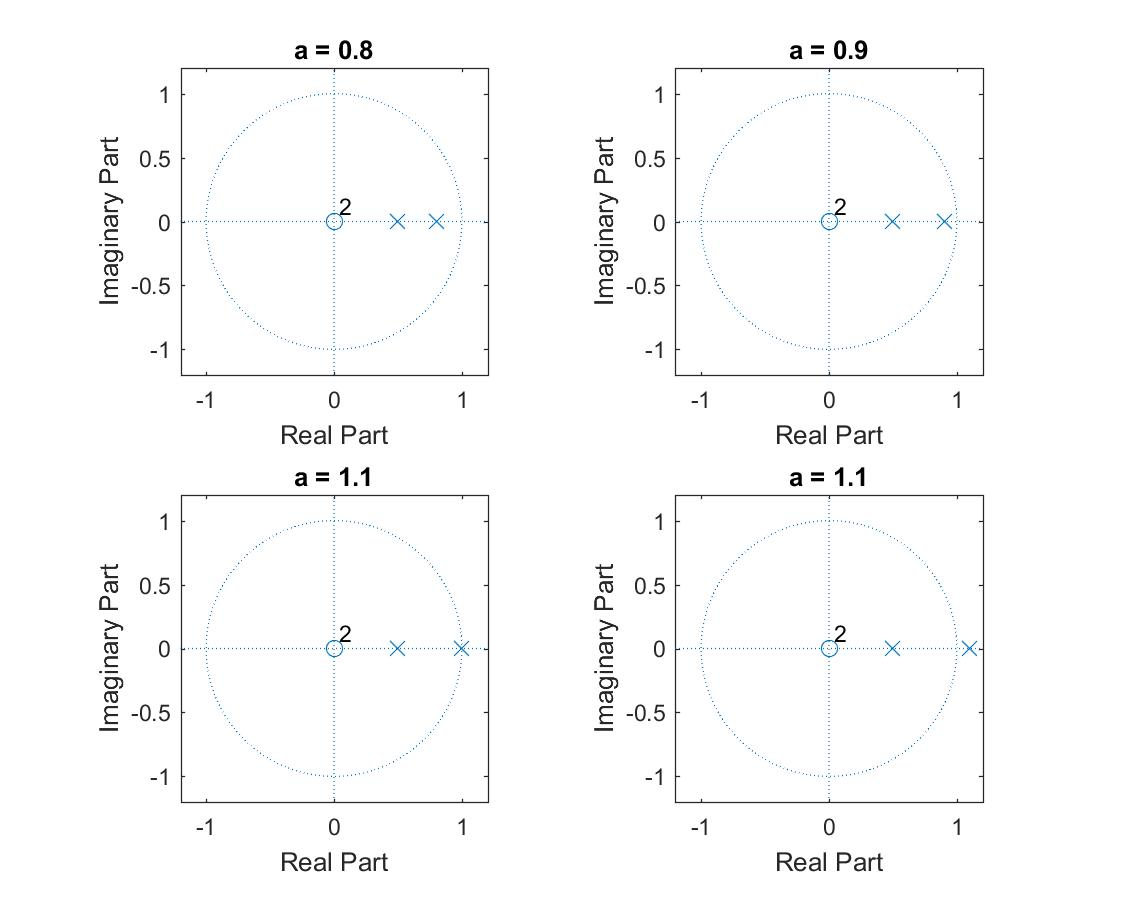
\includegraphics[width=0.6\linewidth]{01.jpg}
                    \caption{系统的零极点分布图}
                    \label{fig:dist}
                \end{figure}
          \item 代码
                \lstinputlisting[language=MATLAB]{code/do.m}
      \end{enumerate}

  \subsection{频率响应}
      $a = 0.8, 0.9, 1.0, 1.1$时,系统的频率响应函数图形及程序如下:
      \begin{enumerate}
          \item 图像如图~\ref{fig:resp} 所示。
                \begin{figure}[!htbp]
                    \centering
                    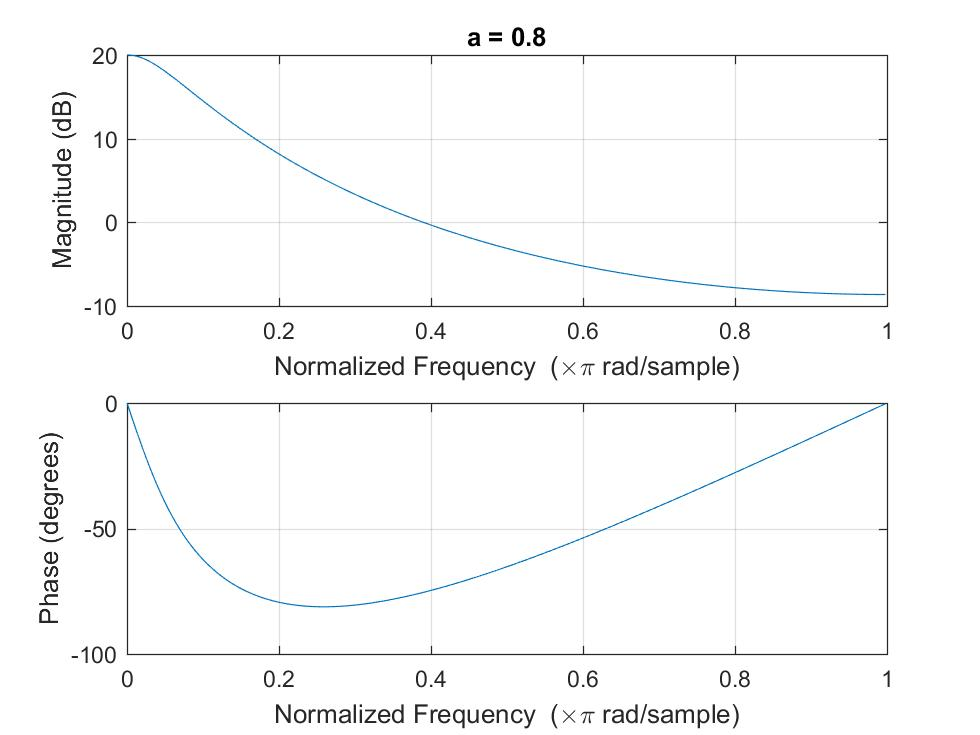
\includegraphics[width=0.6\linewidth]{02-1.jpg}
                    \caption{系统的频率响应函数图形}
                    \label{fig:resp}
                \end{figure}
          \item 代码
                \lstinputlisting[language=MATLAB]{code/next.m}
      \end{enumerate}

      
% 6
\section{实验结果与分析}
...


\end{document}
